\documentclass[../main.tex]{subfiles}

\begin{document}
\chapter{Rozwiązywanie równania renderingu}

\section{Wstęp}

Równanie renderingu (ang. \textit{render equation}) zawiera całkę postaci:

\[
  \int_{\Omega} {
    L(\omega_{l})
    f_r(\omega_{v}, \omega_{l})
    \cos \theta_{l}
    d\omega_{l}
  }
\]

Większość obecnie produkowanych silników do gier używa uproszczenia
polegającego na zastosowaniu świateł punktowych, stąd natężenie światła
przychodzącego jest niezerowe tylko w kierunkach będących znormalizowanymi
wektorami między oświetlanym punktem a każdym z aktywnych świateł w scenie.
Powoduje to, że możemy zredukować powyższą całkę do sumy skończonej:

\[ \sum_{l \in L} L(\omega_l) f_r(\omega_v, \omega_l)\cos \theta_l \]

Obliczenie powyższej sumy, nie jest wyzwaniem dla obecnych kart graficznych
nawet dla większej liczby świateł, szczególnie przy zastosowaniu specjalnych
technik zmniejszających wymaganą liczbę operacji do minimum, np.
\textit{deferred shading}.

W przypadku świateł zajmujących ciągły fragment dziedziny sferycznej, całka nie
może zostać w bezpośredni sposób uproszczona do postaci sumy skończonej bez
utraty dokładności. Niestety również dla większośći funkcji $L$, $f_r$
rozwiązanie dokładne nie będzie możliwe do znalezienia w ograniczonym czasie
wymaganym do zachowania płynności aplikacji.

Metody stosujące niebezpośrednie podejście do wyznaczenia przybliżenia wartości
tej całki zostaną opisane w kolenyhch rozdziałach. Wiedza na temat uzyskania
przybliżenia oryginalnej całki przyda nam się do ich zrozumienia oraz
weryfikacji poprawności.

\section{Metoda Monte Carlo}

Całkowanie czynnika równania renderingu:

$$
\int_{\Omega} {
    L_i(l)
    \rho(l,v)
    \cos \theta_{l}
    \: dl
} $$

\noindent nie jest prostym zadaniem do wykonania. Z pomocą przychodzi metoda
przybliona Monte Carlo bazująca na rachunku prawdopodobieństwa i prawie
wielkich liczb. Metoda dokładnie opisana jest w publikacjach
\cite{MonteCarloAnderson}\cite{Veach}.

\vspace{1cm}
\todo[inline]{Definicje zmiennych losowych? Może to przesada.}
\vspace{1cm}

Dystrybuanta (ang. \textit{cumulative distribution function}, \textit{CDF})
wyznacza prawodpodobieństwo, że zdarzenie losowe $\mathbb{X}$, które zachodzi
ma wartość $\eta$ nie przekraczającą $x$.

$$
F(x) = P(\mathbb{X} \leq x)
$$

Funkcją gęstości prawopodobieństwa (ang. \textit{probability density
function}, \textit{PDF}) nazywamy pochodną dystrybuanty:

$$
f_{\mathbb{X}}(x) = \frac{dF}{dx}(x)
$$

Weżmy funkcję gęstości prawdopobieństwa $f_{\mathbb{X}}$ ciągłej zmiennej
losowej $\mathbb{X}$. Wartość oczekiwana funkcji $g$ na ciągłej zmiennej
losowej $\mathbb{X}$ wynosi:

$$
\mathbb{E}(g(x)) =
\int_{\mathbb{X}}{
  g(x) f_{\mathbb{X}}(x)
  \: dx
}
$$

Estymatorem Monte Carlo przybliżającym wartość $\mathbb{E}(g(x))$ opartym na
prawie wielkich liczb nazywamy:

\[
\widetilde{g_n}(x) =
  \frac{1}{n}
  \sum_{i=1}^{n}g(x_i)
\]

\noindent gdzie, $x=(x_1, \ldots, x_n)$ jest zbiorem $n$ próbek zmiennej
losowej $\mathbb{X}$.

\section{Generowanie próbek}

Próbki Monte-Carlo można wybierać w sposób całkowicie losowy (rys.
\ref{fig:RandomSamples}, jednak taka metoda nie daje nam żadnej gwarancji, że
wybrane próbki będą pokrywały dziedzinę w sposób równomierny. Z pomocą
przychodzą nam ciągi \textit{quasi-losowe}, które pokrywają zadaną dziedzinę w
sposób całkowity i równomierny. Załóżmy, że nasza dziedzina jest kostką $n$
wymiarową: $[0,1]^{n}$.

\begin{figure}[h]
  \centering
  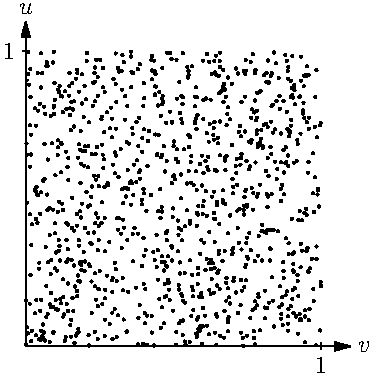
\includegraphics[height=5cm]{montecarlo/random_seq.pdf}
  \caption{Próbki wygenerowane w sposób losowy (1024 próbek)}
  \label{fig:RandomSamples}
\end{figure}

Pierwszą metodą jednorodną jaka się narzuca jest zbudowanie równomiernej siatki
posiadającej $m$ punktów na boku kostki. Problemem tej metody jest jej zbyt
duża jednorodność, wybrane punkty są ułożone w bardzo precyzyjny sposób. Drugim
problemem w niektórych aplikacjach jest ograniczoność metody, zdefiniowaliśmy
dokładnie $m^{n}$ punktów, które musimy wykorzystać, aby zbiór mógł być uważany
za jednorodny, nie możemy punktów usuwać ani dodawać.

\begin{figure}[h]
  \centering
  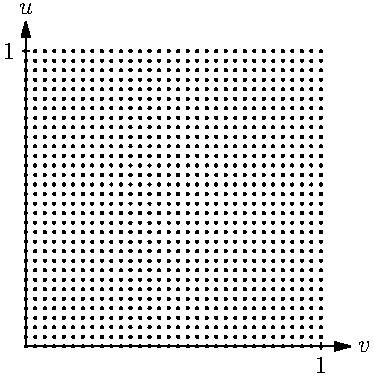
\includegraphics[height=5cm]{montecarlo/uniform_seq.pdf}
  \caption{Próbki wygenerowane przez równomierny podział (1024 próbek)}
  \label{fig:UniformSamples}
\end{figure}

Ciągi o niskiej rozbieżności są rozwiązaniem tego problemu, są to ciągi
deterministyczne, które wydają się losowe przez co posiadają ich zalety oraz
pokrywają równomiernie całą dziedzinę niezależnie od wybranej ilości punktów.

Najbardziej znanymi ciągami tego typu jest ciąg \textit{van der Corput'a} oraz
jego pochodne czyli ciąg Haltona, zbiór Hammersleya.

\subsection{Ciąg van der Corput'a}

Ciąg van der Corput'a \cite{WongSamplingWH} jest jednowymiarowym ciągiem o
niskiej rozbieżności zdefiniowanym na zbiorze $[0,1]$ zbudowanym poprzez
odwrócenie bazy reprezentacji w danym systemie o podstawie $b$. Każda liczba
całkowita $i$ może zostać przedstawiona w pewnej zadanej bazie w sposób
następujący:

\[ i = \sum_{j=0}^{\infty} {a_j b^j} \]

Ciąg van der Corputa transformuje powyższą reprezentację $a_k$, dla $n$-tego
elementu ciągu mamy:

\[ v(n) = \sum_{j=0}^{\infty} {a_j b^{-j-1}} \]

\begin{example}

  Weźmy liczbę $7$ i bazę $2$. Reprezentacja tej liczby może zostać rozpisana
  jako (bez zer nieznaczących):

  \[ 7 = 1 * 2^0 + 1 * 2^1 + 1 * 2^2 = (111)_{b} \]

  \noindent Zatem:

  \[
    v_{2}(7)
      = \frac{1}{2^{1}} + \frac{1}{2^{2}} + \frac{1}{2^{3}}
      = \frac{1}{2} + \frac{1}{4} + \frac{1}{8}
      = 0.875
      \in (0,1)
  \]

\end{example}

Warto zauważyć, że $\sum_{n=1}^{\infty} \frac{b-1}{b^n} = 1$ dla $b>1$.

Kod realizujący powyższe zadanie może być zapisany w formie:

\begin{lstlisting}[language=c++]
double VanDerCorput(unsigned int n, unsigned int base) {
  auto denominator = 1.0;
  auto result = 0.0;

  while (n > 0) {
    denominator /= base;
    result += denominator * (n % base)
    n /= base;
  }

  return result;
}
\end{lstlisting}

Istnieje alternatywne rozwiązanie korzystające z właściwości operacji takiej
odwrotności. Warto zauważyć, że obie liczby $n$ oraz $v(n)$ zapisane w systemie
o podstawie $b$ (tutaj $b=2$) są odbiciem lustrzanym:

\[
  5 = 1 + 4 = (101.0)_{b} \quad
  (0.101)_{b} = 0.625 = \frac{1}{2} + \frac{1}{8} = v(5)
\]

Dla $b=2$ odpowiednio skonstruowana operacja bitowa tego typu pozwoli na
uzyskanie poprawnego wyniku i zwiększenie wydajności obliczeń
\cite{dammertz_2012}\cite{MultidimensionalSampling}:

\begin{lstlisting}[language=c++]
double VanDerCorputRadicalInverse(unsigned int bits)
{
	bits = (bits << 16) | (bits >> 16);
	bits = ((bits & 0x00ff00ff) <<  8) | ((bits & 0xff00ff00) >>  8);
	bits = ((bits & 0x0f0f0f0f) <<  4) | ((bits & 0xf0f0f0f0) >>  4);
	bits = ((bits & 0x33333333) <<  2) | ((bits & 0xcccccccc) >>  2);
	bits = ((bits & 0x55555555) <<  1) | ((bits & 0xaaaaaaaa) >>  1);

	return (double) bits / (double) 0x100000000LL;
}
\end{lstlisting}

\subsection{Ciąg Haltona}

Ciąg Haltona jest uogólnieniem ciągu \textit{van der Corput}'a do wyższych
wymiarów. Weźmy $n$ wzajemnie względnie pierwszych liczb $b_i$ większych od 1,
czyli takiego zbioru w którym dla dowolnej pary liczb ich jedynym wspólnym
dzielnikiem jest 1.

$i$-ty $n$-wymiarowy element ciągu Haltona równy jest:

\[ x(i) = \left( v_{b_0}(i), v_{b_1}(i), \cdots, v_{b_n}(i) \right) \]

\begin{figure}[h]
  \centering
  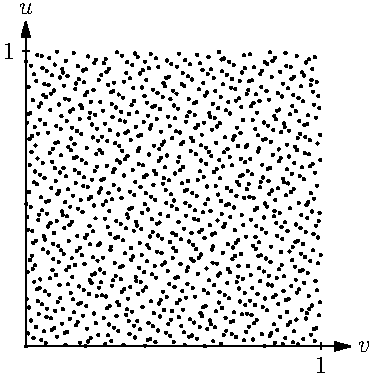
\includegraphics[height=5cm]{montecarlo/halton_seq.pdf}
  \caption{Ciąg Haltona (1024 próbek)}
  \label{fig:HaltonSamples}
\end{figure}

\subsection{Zbiór Hammersleya}

Zbiór Hammersleya jest ciągiem bardzo podobnym do ciągu Haltona, również
korzystającym z ciągu van der Corputa. Chcemy wygenerować $m$ punktów, weźmy
$n-1$ wzajemnie względnie pierwszych liczb $b_i$ większych od 1. $i$-tym $n$
wymiarowym elementem ciągu jest:

\[
  x(i) = \left(
    \frac{i}{m}, v_{b_0}(i), v_{b_1}(i), \cdots, v_{b_{n-1}}(i)
  \right)
\]

Warto zauważyć, że dla wielu parametryzacji potrzebujemy jedynie dwuwymiarowej
parametryzacji, a w takim przypadku bardzo wygodnie jest skorzystać z wersji
bitowej do generowania ciągu van der Corputa, a drugi z parametrów wziąć z
prostej proporcji. Ten zbiór będzie wykorzystywany w kodzie pracy.

\begin{figure}[h]
  \centering
  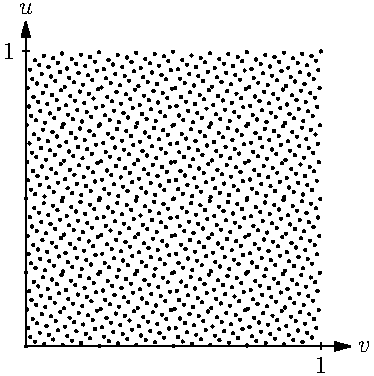
\includegraphics[height=5cm]{montecarlo/hammersley_seq.pdf}
  \caption{Zbiór Hammersleya (1024 próbek)}
  \label{fig:HammersleySamples}
\end{figure}

\subsection{Generowanie próbki z funkcji gęstości prawdopodobieństwa}

Weźmy funkcję gęstości prawdopodobieństwa $f(x)$. Jej dystrybuanta jest równa:

\[ F(s_x) = \int_{-\infty}^{s_{x}} f(x) dx \in [0,1] \]

Załóżmy, że mamy do dyspozycji parametr $\xi \in [0,1]$ wygenerowany dowolną
metodą. Zbudujmy równanie w którym nieznaną zmienną będzie $s_x$:

\[ F(s_x) = \xi \]

Rozwiązując powyższe równanie otrzymamy funkcję odwrotną generującą próbkę
$s_x$:

\[ s_x = F^{-1}(\xi) \]

\subsection{Generowanie punktów na sferze}

Do wygenerowania punktów na sferze możemy wykorzystamy parametryzację:
  $(u,v) \in [0,1]^2 \rightarrow (\theta, \phi) \in \mathcal{H}$

Przekształcenie bezpośrednie tj.:

\begin{align*}
	\theta &= \pi u \\
  \phi &= 2 \pi v
\end{align*}

\noindent nie będzie wystarczające, otrzymany rozkład nie będzie równomierny
\cite{WolframSpherePointPicking}.

Możemy wykorzystać do tego parametryzację jednorodną \cite{dammertz_2012}
\todo{Dopisać wyjaśnienie dlaczego, trójkąt i kąt, rysunkowo}
\todo{Przeczytać: Advanced Computer Graphics Rendering Equation}.

\begin{align*}
	\phi &= \cos^{-1}(1-u) \\
	\theta &= 2 \pi v
\end{align*}

Lub przekształcenie kosinusowe:

\begin{align*}
  \phi &= \cos^{-1}(\sqrt{1-u}) \\
  \theta &= 2 \pi v
\end{align*}


\section{Przyrostowa metoda Monte-Carlo}

Metoda Monte-Carlo ze względu na swoją złożoność obliczeniową nie umożliwia
uzyskania rezultatu w czasie rzeczywistym. Możliwość operowania sceną,
precyzyjnego ustawienia kamery i obiektów nie jest łatwe w takim środowisku.
Czasami nie potrzebujemy również bardzo dużej szczegółowości, czasem wystarczy
nam konkretna ilość iteracji do znalezienia problemu i głównych różnic.

Wygodnym kompromisem jest podzielenie obliczeń na wiele etapów, z których każdy
może zostać wyświetlony jako częściowy podgląd. Dłuższy czas oczekiwania bez
zmian w scenie pozwala nam uzyskać większą jakość.

Spróbujmy zbudować ciąg podsum Monte-Carlo:

\[ I_n = \frac{1}{n} \sum_{i=1}^{n} f(x_i) \]
\[
  I_{n+1} = \frac{1}{n+1} \sum_{i+1}^{n+1}f(x_i)
    = \frac{n}{(n+1)n} \sum_{i=1}^{n}f(x_i) + \frac{1}{n+1}f(x_{n+1})
    = \frac{n}{n+1} I_{n} + \frac{1}{n+1}f(x_{n+1})
\]

Dodatkowy czas potrzebny na przygotowanie ramki, policzenie sumy ważonej i
wyświetlenie rezultatu na ekranie sprawia, że uzyskamy szybszą zbieżność przez
zgrupowanie próbkek w pakiety, które mogą zostać potencjalnie policzone
jednocześnie. Okazuje się, że rozpisanie analogicznego równania dla paczek
danego, stałego rozmiaru jest trywialne:

\begin{align*}
  I_{(m+1)n} &= \frac{1}{(m+1)n} \sum_{i=1}^{(m+1)n} f(x_i)
  = \frac{1}{(m+1)n} \sum_{i=1}^{mn} f(x_i)
    + \frac{1}{(m+1)n} \sum_{i=mn+1}^{(m+1)n} f(x_i) = \\
  &= \frac{m}{(m+1)mn} \sum_{i=1}^{mn} f(x_i)
    + \frac{1}{(m+1)n} \sum_{i=mn+1}^{(m+1)n} f(x_i) \\
  &= \frac{m}{m+1}I_{mn}
    + \frac{1}{m+1} \left(
        \frac{1}{n} \sum_{i=mn+1}^{(m+1)n} f(x_i)
    \right)
\end{align*}

Powyższe obliczenie sumy ważonej może zostać zrealizowane za pomocą sprytnie
zbudowanego łańcucha \textit{framebufferów} i obliczone za pomocą wspartego
sprzętowo mechanizmu łączenia kolorów (ang. \textit{blending}). Obecna partia
musi zostać obliczona do jednego z buforów oraz skopiowana z włączonym
mieszaniem kolorów do drugiego bufora. Można zastosować uproszczenie, w którym
wykorzystamy tylko jeden bufor, ale czasami ze względu na istnienie wielu
świateł i wybraną technikę (np. \textit{deferred shading}) może być koniecznie
zastosowanie dwóch buforów.

\section{Importance Sampling}

Importance Sampling jest jedną z metod ograniczania wariancji metody
Monte-Carlo. Innymi słowy, zastosowanie tej techniki poprawnie powinno
skrócić czas w którym ciąg zbiegnie do odpowiednio bliskiej wartości całki.

Publikacje \cite{Veach}\cite{MonteCarloAnderson} sugerują zastosowanie innej
techniki generowania próbek, tak aby większość z nich była generowana w
miejsach które są istotne dla wyniku.

Mając funkcję gęstości zmiennej losowej $\mathbb{X}$ $h(x)$ na której potrafimy
całkować, wyznaczać jej wartość w punkcie oraz jest prawie proporcjonalna do
całkowanej funkcji $g(x)$ możemy przepisać:

\[
  \int_{x \in \mathbb{A}} { g(x) dx } =
  \int_{x \in \mathbb{A}} { g(x) \frac{h(x)}{h(x)} dx } =
  \int_{x \in \mathbb{A}} { \frac{g(x)}{h(x)} h(x) dx } =
  \mathbb{E}_{h}\left({ \frac{g(x)}{h(x)} }\right)
\]

Jeżeli funkcja gęstości prawdopodobieństwa $h(x)$ zostanie wybrana mądrze to
wariancja estymatora Monte-Carlo zmniejszy się. Aby funkcja $h(x)$ była
użyteczna, musi spełniac kilka warunków:

\begin{itemize}

  \item obliczenia dotyczące funkcji $h$ muszą być łatwo realizowalne,
    obliczenie wartości funkcji, jej całki musi być możliwe bez wykorzystania
    metody Monte-Carlo

  \item symulowanie próbek z rozkładu $h$ musi być realizowalne

  \item $h(x) > 0$ dla $g(x) \neq 0$

  \item $h(x)$ musi być możliwie proporcjonalne do $|g(x)|$, inaczej wariancja
    zamiast zmaleć, wzrośnie

\end{itemize}

Teoretycznie najlepszym wyborem jest funkcja $g'(x) = cg(x)$ gdzie:

\[
c \propto \frac{1}{\int_{\Omega}{g(x)dx}}
\]

\noindent Niestety, taka funkcja jest niemożliwa do wykorzystania praktycznego
w sposób bezpośredni, ponieważ mianownik w stałej $c$ jest naszą szukaną całką,
której przecież nie potrafimy policzyć. Będziemy szukać funkcji $h$ podobnych
kształtem do $g$.

Istotnym problemem tej metody jest to, że nieuważny wybór funkcji $h$ może
znacząco pogorszyć wariancję (rys. \ref{fig:ImportanceSamplingProblems}.

\begin{figure}
  \centering

  \begin{subfigure}[t]{0.45\textwidth}
    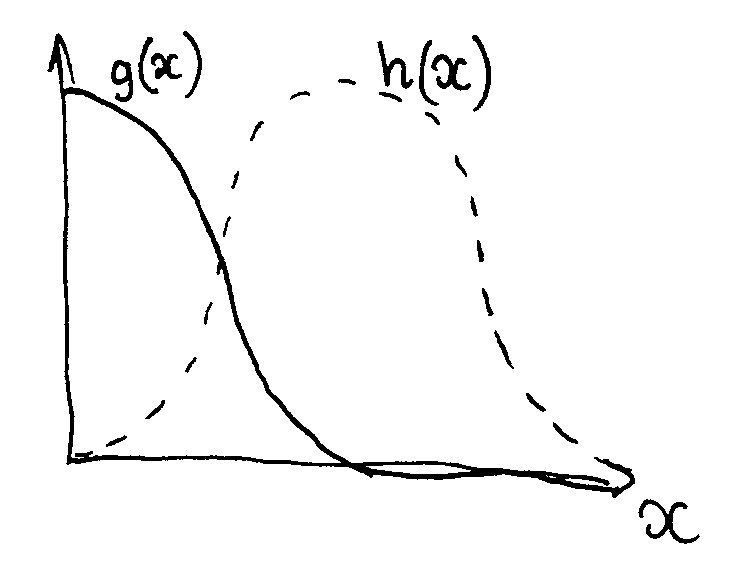
\includegraphics[width=\textwidth]{montecarlo/is_different_shape.jpg}
    \label{fig:ImportanceSamplingWrongFunction}
    \caption{Nie odwzorowany kształt estymowanej funkcji}
  \end{subfigure}
  \begin{subfigure}[t]{0.45\textwidth}
    \centering
    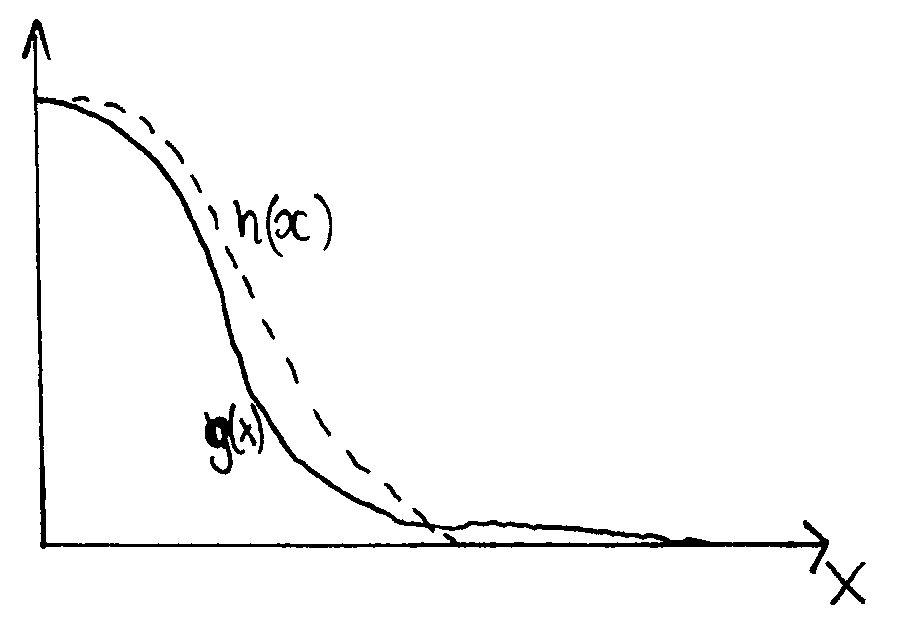
\includegraphics[width=\textwidth]{montecarlo/is_lost_tail.jpg}
    \label{fig:ImportanceSamplingLostTail}
    \caption{Nie uwzględnienie ,,ogona'' rozkładu}
  \end{subfigure}

  \label{fig:ImportanceSamplingProblems}
  \caption{Przykłady problemów związanych z wyborem $h(x)$}
\end{figure}

\section{Importance Sampling dla poszczególnych rodzajów BRDF}

Pozostaje jeszcze kwestia znalezienia konkretnej funkcji $h(x)$ z której
będziemy mogli skorzystać przy Importance Samplingu. Po pierwsze funkcja
ma mieć podobny kształt do funkcji podcałkowej oraz musimy potrafić wygenerować
próbkę.

\subsection{Phong BRDF}

Znajdźmy funkcję gęstości prawdopodobieństwa nadającą się do generowania próbek
dla BRDF Phonga
  \cite{NotesImportanceSampling} \cite{ImportanceSamplingForProduction}:

\[
  L_o(\omega_o) = \int_{\Omega} {
    L_i(\omega_i) \cos^{n}\theta_s \cos\theta_i d\omega_i
  }
\]

Będziemy poszukiwać funkcji $p(\theta, \phi)$:

\noindent z której będziemy mogli wygenerwować próbki korzystając z funkcji
odwrotnych:

\begin{align*}
  s_\theta &= F_{\theta}^{-1}(\xi_\theta) \\
  s_\phi &= F_{\phi}^{-1}(\xi_\phi)
\end{align*}

\noindent użytecznych do oszacowania całki:

Interesuje nas część $\cos^{n}\theta_s$ w odniesieniu do kąta bryłowego
$d\omega_i$.

Wykorzystajmy tą funkcję jako kształt dla szukanej funkcji gęstości
prawdopodobieństwa. Funkcja gęstości $p(x)$ musi spełniać warunek:

\[ \int_{-\infty}^{\infty} p(x) dx = 1 \]

\noindent stąd (czynnik $\sin\theta$ pochodzi z zamiany do współrzędnych
sferycznych z kątów bryłowych:

\[
  p(\theta, \phi) = \frac{
    \cos^{n}{\theta} \sin\theta
  }{
    \int_{0}^{2\pi} \int_{0}^{\frac{\pi}{2}} {
      \cos^{n}{\theta} \sin\theta d\theta
    }
  }
\]

Rozwiązując poniższą całkę otrzymujemy poniższy dwuwymiarowy rozkład gęstośći
prawdopodobieństwa (patrz listing \ref{appendix:maxima_phong}):

\[
  p(\theta, \phi) =
    \frac{n+1}{2\pi} \cos^{n}\theta \sin\theta
\]

Rozbijmy zmienne $\theta$ oraz $\phi$ na dwie oddzielne niezależne funkcje
korzystając z rozkładu brzegowego (ang. \textit{marginal density function}):

\[
  p(\theta) = \int_{0}^{2\pi} {
    p(\theta, \phi) d \theta
  } =
  (n+1) \cos^{n}{\theta} \sin\theta
\]

Korzystając z twierdzenie Bayesa możemy obliczyć rozkład warunkowy
	$p(\phi | \theta)$:

\[
  p(\phi | \theta) = \frac{
    p(\theta, \phi)
	}{
		p(\theta)
	} = \frac{1}{2\pi}
\]

Oba rozkłady konwertujemy do postaci dystrybuanty którą będziemy próbkować
korzystając ze zmiennych losowych $(\xi_{\theta}, \xi_{\phi}) \in [0,1]^2$:

\[
	\xi_1 = P(s_{\phi}) =
	\int_{0}^{s_{\phi}} {
		p(\phi) d\phi
	} =
	\int_{0}^{s_{\phi}} {
		\frac{1}{2\pi}
	} =
	\frac{s_{\phi}}{2\pi}
\]

Stąd możemy wyznaczyć:

\[
	s_{\phi} = 2 \pi \xi_{\phi}
\]

Analogicznie postępujemy z rozkładem brzegowym:

\[
  \xi_{\theta} = P(s_{\theta}) =
	\int_{0}^{s_{\theta}} {
		p(\theta) d\theta
	} =
	\int_{0}^{s_{\theta}} {
		\frac{n+1}{2\pi} \cos^{n}\theta \sin\theta d\phi
	} =
	1 - \cos^{n+1}(s_{\theta})
\]

Z czego mamy:

\[
	s_{\theta} =
	\cos^{-1}\left[
		(1 - \xi_{\theta})^{\frac{1}{n+1}}
	\right]
\]

lub ze względu na losowość rozkładu (rozkład uzyskany przez lustrzane odbicie
dalej jest losowy i spełnia wszystkie założenia):

\[
	s_{\theta} =
	\cos^{-1}\left(
		\xi_{\theta}^{\frac{1}{n+1}}
	\right)
\]

\subsection{Trowbridge-Reitz BRDF (GGX)}

\[
  \int D(m) (n \cdot m) dm = \left(\int D(m) cos\theta dm\right) = 1
\]

NDF:

\[
	D(m) = \frac{
		\alpha^2
	}{
    \pi \left(
      \cos^{2}(n \cdot m)(\alpha^2 - 1) + 1
    \right)^{2}
  }
\]

\[
  p(\theta, \phi) =
	\frac{
    \alpha^2 \cos\theta \sin\theta
	}{
    \pi \left(
      \cos^{2}\theta (\alpha^2 - 1) + 1
    \right)^{2}
  }
\]

Analogicznie do poprzedniego przykładu oba rozkłady konwertujemy do postaci
dystrybuanty którą będziemy próbkować korzystając ze zmiennych losowych
  $(\xi_{\theta}, \xi_{\phi}) \in [0,1]^2$:

\[
  p(\theta) = \int_{0}^{2\pi} {
    p(\theta, \phi) d \theta
  } =
  \frac{2 \alpha^2 \cos\theta \sin\theta}{
    \left(
      \cos^{2}\theta (\alpha^2 - 1) + 1
    \right)^{2}
  }
\]

Dla $\phi$ proces wygląda analogicznie do BRDF Phonga:

\[
  p(\phi | \theta) = \frac{
    p(\theta, \phi)
	}{
		p(\theta)
	} = \frac{1}{2\pi}
\]

\[
	\xi_\phi = P(s_{\phi}) =
	\int_{0}^{s_{\phi}} {
		p(\phi) d\phi
	} =
	\int_{0}^{s_{\phi}} {
		\frac{1}{2\pi}
	} =
	\frac{s_{\phi}}{2\pi}
  \Rightarrow
	s_{\phi} = 2 \pi \xi_{\phi}
\]

\[
  \xi_\theta = P(s_{\theta}) =
	\int_{0}^{s_{\theta}} {
		p(\theta) d\theta
	} =
  2 \alpha^2 \left(
    \frac{1}{
      (2\alpha^4 - 4\alpha^2 + 2) \cos^{2}{s_\theta} + 2\alpha^2 - 2
    } - \frac{1}{
      2\alpha^4 - 2\alpha^2
    }
  \right)
\]

Po przekształceniu powyższego wzoru uzyskujemy:

\begin{align*}
  s_\theta &= \cos^{-1}\left(
    \sqrt{
      \frac{1 - \xi_\theta}{\alpha^2 \xi_\theta - \xi_\theta + 1}
    }
  \right) \\
  s_{\phi} &= 2 \pi \xi_{\phi}
\end{align*}

\subsection{Rozkłady wykładnicze}

Nie wszystkie rozkłady mogą być rozwiązane korzystając z powyższej metody.
Box-Muller.

\section{Multiple Importance Sampling}
\label{Chapter:MIS}

Załóżmy, że mamy $n$ różnych funkcji gęstości prawodpodobieństwa $p_{i}(x)$ dla
$i \in \{ 1, \cdots, n \}$ opisujących istotność poszczególnych próbek dla
danych czynników szukanej funkcji $f(x)$. Każda z tych strategii działa lepiej
w pewnych obszarach dziedziny, jednakże gorzej od nich w każdym innym miesjcu.
Chcielibyśmy dynamicznie wybierać, której strategii używać w danym momencie,
tak aby wariancja spadła jeszcze bardziej.

Naiwnym podejściem jest obliczenie całki korzystając z każdego z podejść
i uśrednienie wyniku, takie podejście nie da nam pożądanego rezultatu.

Zbudujemy model wielopróbkowy (ang. \textit{multi-sample model})
\cite{pbrt}\cite{ImportanceSamplingForProduction} korzystający z wygenerowanych
próbek z wielu źródeł jednocześnie, których wyniki będą mieszane zgodnie z
pewną funkcją mieszającą $w$. Nasz estymator Monte-Carlo będzie wyglądał
następująco:

\[
  F = \sum_{i=1}^{n} \frac{1}{n_i} \sum_{j=1}^{n_i} w_{i}(X_{i,j}) \frac{
    f(X_{i,j})
  }{
    p_{i}(X_{i,j})
  }
\]

Aby estymator $F$ pozsotał \textit{unbiased} funkcja $w_i$ musi spełniać
następujące warunki:
% MIS p.261

\[ \sum_{i = 1}^{n} w_{i}(x) = 1 \text{ dla } f(x) \neq 0 \]
\[
  \forall i \in \{ 1, \ldots, n \} \quad
  w_{i}(x) = 0 \Leftrightarrow p_i(x) = 0
\]

Za najlepsze funkcją mieszającą $w_i$ sprawdzające się w większości zastosowań
uważa się funkcje postaci:

\[
  w_{i}(x) = \frac{
    n_{i} p_{i}(x)
  }{
    \sum_{k=1}^{n} {
      n_{k} p_{k}(x)
    }
  }
\]

\noindent nazywane heurystyką balansującą (ang. \textit{balance heuristics}).

\end{document}
